

%************************************************
\chapter{The Information Bottleneck and Deep Learning}\label{ch:ib_and_dl}

%************************************************
\begin{quotation}
	\small \textit{ \flushright
	Great claims require great evidence.
	\flushright --- Carl Sagan \\
	\vspace{1cm}}
\end{quotation}


This chapter presents:
% - ### IB and Deep Learning
% 	- #### Types of works on IB in DL (Intro)
% 		- ##### DNN analysis/criticism
% 		- ##### Applications
% 			- IB based algorithms
% 			- Transfer Learning
% 		- ##### IB theory of DL
% 	- #### DNN analysis/criticism
% 		- IB as X-ray
% 		- Saxe et al.
% 		- Goldferb et al.
% 		- Deep Invertible networks
% 		- M.I. measurement
% 		- Invertible Deterministic function: $H(T)=H(X)$
% 		- "It is a known fact that the IB is ill-posed for deterministic (...)", Tishby video
% 		- stochastic function?
% 		- Quantization, computers
% 		- Dataset has some stochasticity
% 	- #### IB based training and algorithms (applications)
% 		-   Achille, Soatto
% 		-   Alemi, Fischer
% 	- #### IB theory of DL
% 		- comparing assumptions
% 		- Shamir, Sabato, Tishby
% 		- Achille, Soatto
% 		- ##### new narrative for explainable phenomena
% 			- ###### flat minima
% 				- Hochreit and Schimdhuber
% 				- MacKay Evidence Framework
% 				- Achille Implicit regularization (Fischer information)
% 			- ###### the role of layers in DL
% 				- Achille misses the point
% 				- original explanation based on IBT
% 		- ##### new explanations for unexplainable phenomena
% 			- ###### Critical Learning Periods
% 			- ###### Super convergence
% 				- (GAP) Research opportunity for original contribution
% 		- ##### Activations vs weights
% 			- ###### duality
% 				- different meanings
% 				- $\min I(D;W) \to \min I(X;T)$, proof by Achille
% 		- ##### Information in the Activations
% 			- ###### deterministic
% 			- ###### In videos, Tishby clearly understand the duality of activation and weights
% 			- ###### Tishby's work mixed analysis with explanations.
% 			- ###### Critics didn't like explanations (of information in the activations. Lack of rigor.) and discarded the analysis
% 		- ##### Information in the weights
% 			- ###### emergence of regularization term
% 				- SGD implicit regularization
% 			- ###### Connection to PAC-Bayes
% 				- vacuous PAC-bayes bounds
% 				- from PAC-Bayes to IB Lagrangian
% 				- Achille aims to show connection, not to suggest new bounds
% 		- ##### Sample bounds on empirical MI
% 			- Shamir, Sobato, Tishby
\section{Types of literature on Information Bottleneck and Deep Learning}
Critics point out that the output of some learning algorithms are invertible deterministic functions and, as such, due to reparametrisation invariance (Theorem \ref{th:reparemetrisation_invariance}), they do not change the amount of information of the input. In these cases, there is no compression, and the amount of information in the representation is equivalent to the input's entropy. Tishby argues that any learning algorithm has noise due to finite computer memory and are not deterministic. Besides, he proposes injecting noise in the running of every \emph{snapshot}, a kind of \emph{test time augmentation}\footnote{\bt{Test time augmentation} is a common practice in ML that injects noise to a test input, by generating transformed versions of it, and combines the predictions of these versions.}, to measure information, which will lead to slightly different $\hat{\ry}_i$  in different runs of the model for the same $\rx_i$.


Despite calling his work \emph{Information Bottleneck Theory}, Tishby admits it is not ``rigorously proven'' theory, and he argues that the initial strong criticism is ``throwing the baby with the water''. For him, the IB should be seen as a tool, an ``X-Ray'', to analyse the behaviour of learning algorithms during training\footnote{In reality, his focus has been on analysing Deep Learning models.  This argument, however, can be applied to any learning algorithm.}~\cite{tishby:2020DeepMath}. For this, he is interested in measuring information in the representation of {input examples} (\emph{information in the activations}) during training. Each sample fed to the training generates a ``snapshot'' of the quality of representations being generated.


\section{IB based analysis of Deep Learning}
In their numerical experiments\cite{shwartz-ziv:2017}, they use unregularized fully connected feed-forward neural networks with hyperbolic tangent hidden layer activation functions, SGD and cross-entropy loss function. To estimate $I[\rvX;\rvZ_L], I[\rvY;\rvZ_i]$, they bean each neuron's double-soded saturation arctan output activation into 30 equal intervals to calculate the mutual information pair over epochs. They produce the information plane over 50 different randomized initializations.  Visual appealing... 2 distinct phases. First, in a shorter empirical error minimization (ERM) phase and a much longer compression phase, $I[\rvX;\rvZ_L]$ gradually decreases. Learning is forgetting. authors suggest this representation compression phase is enabled by SGD's diffusion-like behavior and responsible fort the generalisation performance.
\subsection{Tishby's main thesis}
Learning is forgetting
Information Plane
\subsection{Criticism to Tishby's main thesis}\label{sec:criticsm}
\citeauthor{shwartz-ziv:2017} results were challenged shortly after by \cite{saxe:2018}. Foremost, \citeauthor{saxe:2018} note that the use of a binning procedure to estimate mutual information is ambiguous, as the true mutual information between $I[\rvX;\rvZ_L]$ is provably infinite for continuous distributions and constant (\ie equal to $H[\rvX])$ for discrete distributions. Reparemetrisation property -> and activation function is invertible transformation (deterministic mapping) of input. The binning injects noise that is external to the network. They replicated the experiment with an identical tanh-actication, but also tried alternative versions with ReLU, softsign and softmax. The ReLU function do not comproess in their experiment. They also take into account that the plotted mutual information results are incluenced by the user-selected nmber of bins and binning strategy. Overall, \citeauthor{saxe:2018} refute \citeauthor{shwartz-ziv:2017} results.
\cite{goldfeld:2019} show that their $I[\rvX;\rvZ_L]$ estimates does not directly measure compression of the true mutual information.
\cite{chelombiev:2018} explore several estimation schemes for measuring compression and propose an entropy-based adaptative binning strategy (EBAB). Under EBAB, the RELU exhibits much more compression. They make the caveat regarding how initialization may affect information plane.
\citeauthor{achille:2017emergence} take a related but different approach. They create their own IB Lagrangian between weights and data. They relate their Lagrangian to PAC-Bayes framework. They propose that information in weights is not only a measure of learned model complexity, but also relates to a transition from underfitting to overfitting.They show that DNNs are not inconsitent with bias-variance trade-off theorem if complexity is interpreted in terms of information rather than dimensionlity. They demonstrate this deriving a cross-entropy loss decompposition.
Hp.q = intrinsic error + sufficiency + efficiency + overfitting

The implicit overfitting term in cross-entropy suggest one can overcome overfitting by adding back the overfitting term.

They also empirically validate 3 main takeawyas: there is a transition from overfitting to underfitting, the bias-variance trade-off holds when interpreted in terms of information and that by decreasing information in the weights representations can be made insensitive to nuances.
.... empirical ....
Achille and Soatto produce a generally satisfying theoretical work.

information-plane visually appealing contribute dto the popularity.. lack theoretical rigor.

Achille and Soatto research, in contraposition, is trying to use the IB framework not only to explain but also to improve learning algorithms.  In their view, noise during training helps generalisation. They argue that the noise in Stochastic Gradient Descent is responsible for Deep Learning generalisation power. Moreover, they believe that generalisation can be further improved by controlled injection of noise during training. They are interested in measuring and \emph{controling} the information in the representation of the task (\emph{information in the weigths}).
- IB as X-ray
		- Saxe et al.
		- Goldferb et al.
		- Deep Invertible networks
		- M.I. measurement
		- Invertible Deterministic function: $H(T)=H(X)$ information is a property of random variables, which may be degenerate for the deterministic pro- cess of computing the output of a trained DNN in response to a given input (inference). Achille and Soatto 2021

		- "It is a known fact that the IB is ill-posed for deterministic (...)", Tishby video
		- stochastic function?
		- Quantization, computers
		- Dataset has some stochasticity
		subsubsection This is a weakness

		- quantization: Because quantization is a many-to-few mapping, it is an inherently non-linear and irreversible process (i.e., because the same output value is shared by multiple input values, it is impossible, in general, to recover the exact input value when given only the output value).
		Assuming neural networks are non-linear non-inversible functions, finite hypothesis space
		The set of possible input values may be infinitely large, and may possibly be continuous and therefore uncountable (such as the set of all real numbers, or all real numbers within some limited range). The set of possible output values may be finite or countably infinite.[6] The input and output sets involved in quantization can be defined in a rather general way. For example, vector quantization is the application of quantization to multi-dimensional (vector-valued) input data. In the typical case, the original signal is much larger than one least significant bit (LSB). When this is the case, the quantization error is not significantly correlated with the signal, and has an approximately uniform distribution.
		- Turing \cite{turing:1936} countable set of all possible computer programs -> set of computable real numbers is also countable -> The set of reals in uncountable -> most reals are uncomputable, infinitely many more than are computable. Algebraic reals can be computed digit by digit.
		- no physical quantity has ever been measured with more than twenty digits of precision\cite[p. 92]{chaitin:2006}
		- philosophical and mathematical argument against the physical existance of real numbers \cite[99-116]{chaitin:2006}
\subsection{The faux plane}
	Experimental results that corroborate to
\section{IB based training and algorithms}
Achille
Alemi, Fischer
\section{IB Theory of Deep Learning}
\subsection{A new narrative for understanding Deep Learning Phenomena}


% \subsection{Possible explanations for unexplained Deep Learning Phenomena}
% Several pleasant features underlay the success of deep learning: The scarcity of bad minima en- countered in their optimization [Draxler et al. (2018); Choromanska et al. (2014)], their ability to generalize well despite being heavily over-parametrized [Neyshabur et al. (2018, 2014)] and expres- sive [Zhang et al. (2016)], and their ability to generate internal representations which generalize across different domains and tasks [Yosinski et al. (2014); Sermanet et al. (2013)]. Our current understanding of these features is however largely empirical.Internal representation are a key ingredient in transfer learning [Yosinski et al. (2014); Sermanet et al. (2013)]
\subsection{Generalization power despite number of parameters}
\subsection{Generalization despite expressiveness--overfitting}
\subsection{ability to generate internal representations which generalise across domains and taks}
\subsection{Scarcity of bad minima encountered in their optimisation}
\begin{figure}[h]
  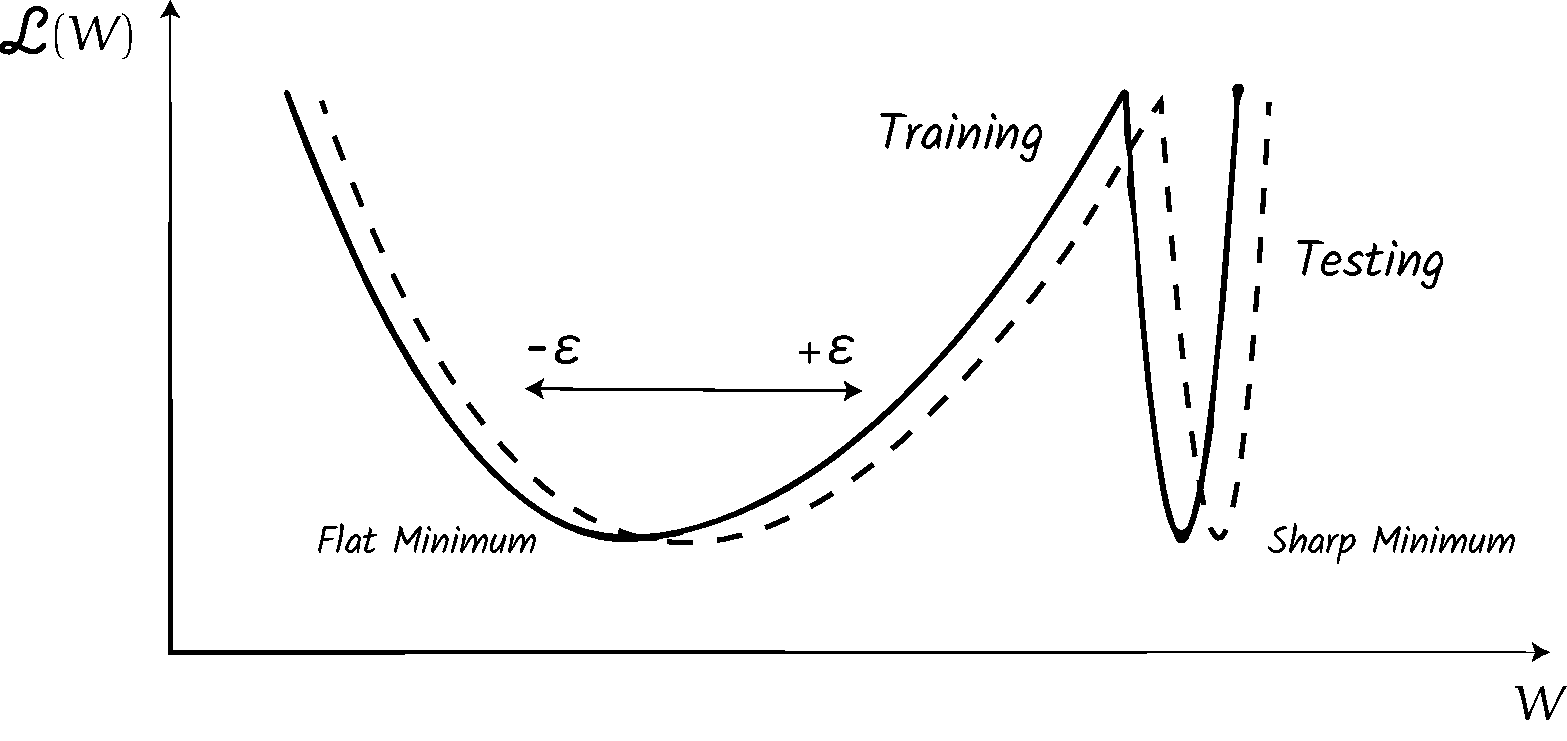
\includegraphics[width=\columnwidth]{flat-minima}
  \caption{Information in the weights explain the preference of SGD for flat minima.}
  \label{fig:flat_minima}
\end{figure}
The relation of low Fisher Information in the weights and good generalization in the activations bring us another interesting insight. It is a well documented phenomena that DNNs trained with SGD tend to find flat minima, meaning saddle points where some noise in the test data will minimally affect the loss (see figure \ref{fig:flat_minima}).  Here we have a theoretical reason why this is happening. SGD is implicitly regularizing the information in the weights and that is the same as looking for minimas with low Fisher Information, which are Flat Minimas.

Hochreiter and Schmidhuber discuss sharp versus flat minima using the language of minimum de- scription length In short, describ- ing weights in sharp minima requires high precision in order to not incur nontrivial excess error, whereas flat min- imum can be described with lower precision. A similar coding argument appears in [HC93].

\subsection{The role of layers in deep learning}
Why do we need multiple layers in a neural network? This question is fundamental in Deep Learning, and still, there is no definitive answer. A feedforward network with a single layer can represent any function\cite{goodfellow:2016}. Also, \cite{leshno:1993} (as cited by \cite{goodfellow:2016}) demonstrated that shallow networks with rectified linear units as activation functions have universal approximation properties. When confronted with these facts, the usual answer for the need for depth is that these results require an infeasible large layer or do not address efficiency. Another common answer is that layers provide levels of abstraction and a paramount composability property, \ie stacking layers allow a network to represent functions of increasing complexity\cite{goodfellow}. These answers seem correct but, at the same time, somewhat qualitative and vague\footnote{Teo: Any reference of quantitative proof for the need for depth?}.

This section will try to advance the discussion by answering the need for depth in Neural Networks with an Information Bottleneck perspective.

We have already established that a DNN optimised with SGD solves an \ac{IB} problem. In this view, the body of the network is an encoder that compresses the input $\rvX$ into a representation $\rvZ$. In the IBT perspective, training  a DNN is finding the encoder that minimises $\IZX$:
\begin{align*}
	Q(\rvZ|\rvX)~|~Q = arg\ min\ \IZX
\end{align*}

From~\cite{achille:2017emergence}:
\begin{corollary}[Bottlenecks promote invariance] Assume a Markov chain of layers:
	\begin{align*}
		\rvX \to \rvZ_1 \to \rvZ_2,
	\end{align*}
and that there is a bottleneck between $\rvZ_1$ and $\rvZ_2$ (for example, if $dim(\rvZ_1)>dim(\rvZ_2)$ or noise has been added between to the channel $\rvZ_1 \to \rvZ_2$ via dropout\footnote{Dimensionality reduction can be seen as a form of noise.}). Then, if $\rvZ_2$ is sufficient, it is more invariant to nuisances than $\rvZ_1$ (see \cref{sec:invariant_if_minimal}).
\end{corollary}

\begin{corollary}[Stacking increases invariance] Assume a Markov chain of layers:
	\begin{align*}
		\rvX \to \rvZ_1 \to \rvZ_2 \to \cdots \to \rvZ_L,
	\end{align*}\label{cor:stacking_layers}
	and that $\rvZ_L$ is sufficient of $\rvX$ w.r.t. $\rvY$. Then, by \ac{DPI}:
	\begin{align*}
		I[\rvZ_L;\rvX] \leq I[\rvZ_i;\rvX], \forall i \in \{1 \cdots L-1\},
	\end{align*}
	therefore $\rvZ_L$ is more insensitive to nuisances than all preceding layers and generalises better.
\end{corollary}

In other words, \citeauthor{achille:2017emergence} argue  that \textbf{stacking layers improve generalisation}.
A problem with this argument is that It only shows that in the multi-layered scenario, the last layer is more compressed and invariant to nuisances. It is not direct that a single-layered network can not achieve the same level of compressibility of the input as the last layer in the multi-layered scenario.

Besides, according to \cite{achille:2017emergence}, the above corollary does not simply imply that the more layers, the merrier, as it assumes that one has successfully trained the network ($\rvZ_L$ is sufficient). For the authors, a successfully trained network becomes increasingly difficult as the network grows.The increase in difficulty seems straightforward because stacking layers increase the number of computations per batch.

By pure logic, it is evident that the complexity of any algorithm that searches for the best possible hypothesis will depend on the size of the hypothesis space. Counterintuitively, however, we claim that \bt{stacking layers decrease the complexity of the training in practice}, as they reduce the ``typical'' hypothesis space size. We argue that stacking layers increase the complexity of the learning algorithm by a constant while exponentially decreasing the size of the ``typical'' hypothesis space.

To explain how stacking layers reduce the ``typical'' hypothesis space size, let us start with the case of a single layer DNN. We need to find:
\begin{align}
	Q_1^* = Q_1(\rvZ_1|\rvX)~|~Q_1^* = arg\ min\ \IZX
\end{align}

What is the ``typical'' hypothesis space in this case? First, let $\sA_{\rvQ_1}$ be the hypothesis space of all functions that encode $\rx \in |\sA_{\rvX}|$ possible inputs into $\rz \in |\sA_{\rvZ}|$ possible outcomes. Nevertheless, from Shannon's Noisy Channel Theorem (\cref{noisy_channel_theorem}) there are only $2^{H[\rvX]}$ typical $\rx_i$ and for each typical $\rx_i$ there is only $2^{H[Z|X]}$ ``typical'' outcomes (see \cref{sec:source_encoding_theorem}), therefore, the number of decodable encodings (one to one mappings) is:
\begin{align}
\forall q \sim \sA_{Q_1},&~Pr(q \in \sA_{Q_1}^\epsilon) = 1 -\epsilon, \epsilon < \dfrac{1}{2}\\
|\sA_{Q_1}^\epsilon| &= \frac{2^{H[\rvX]}}{2^{H[\rvZ_1|\rvX]}}=2^{\IZX}.
\end{align}
where $\epsilon$ can be arbitrarily small.
\begin{figure}
	[ht!] \centering
	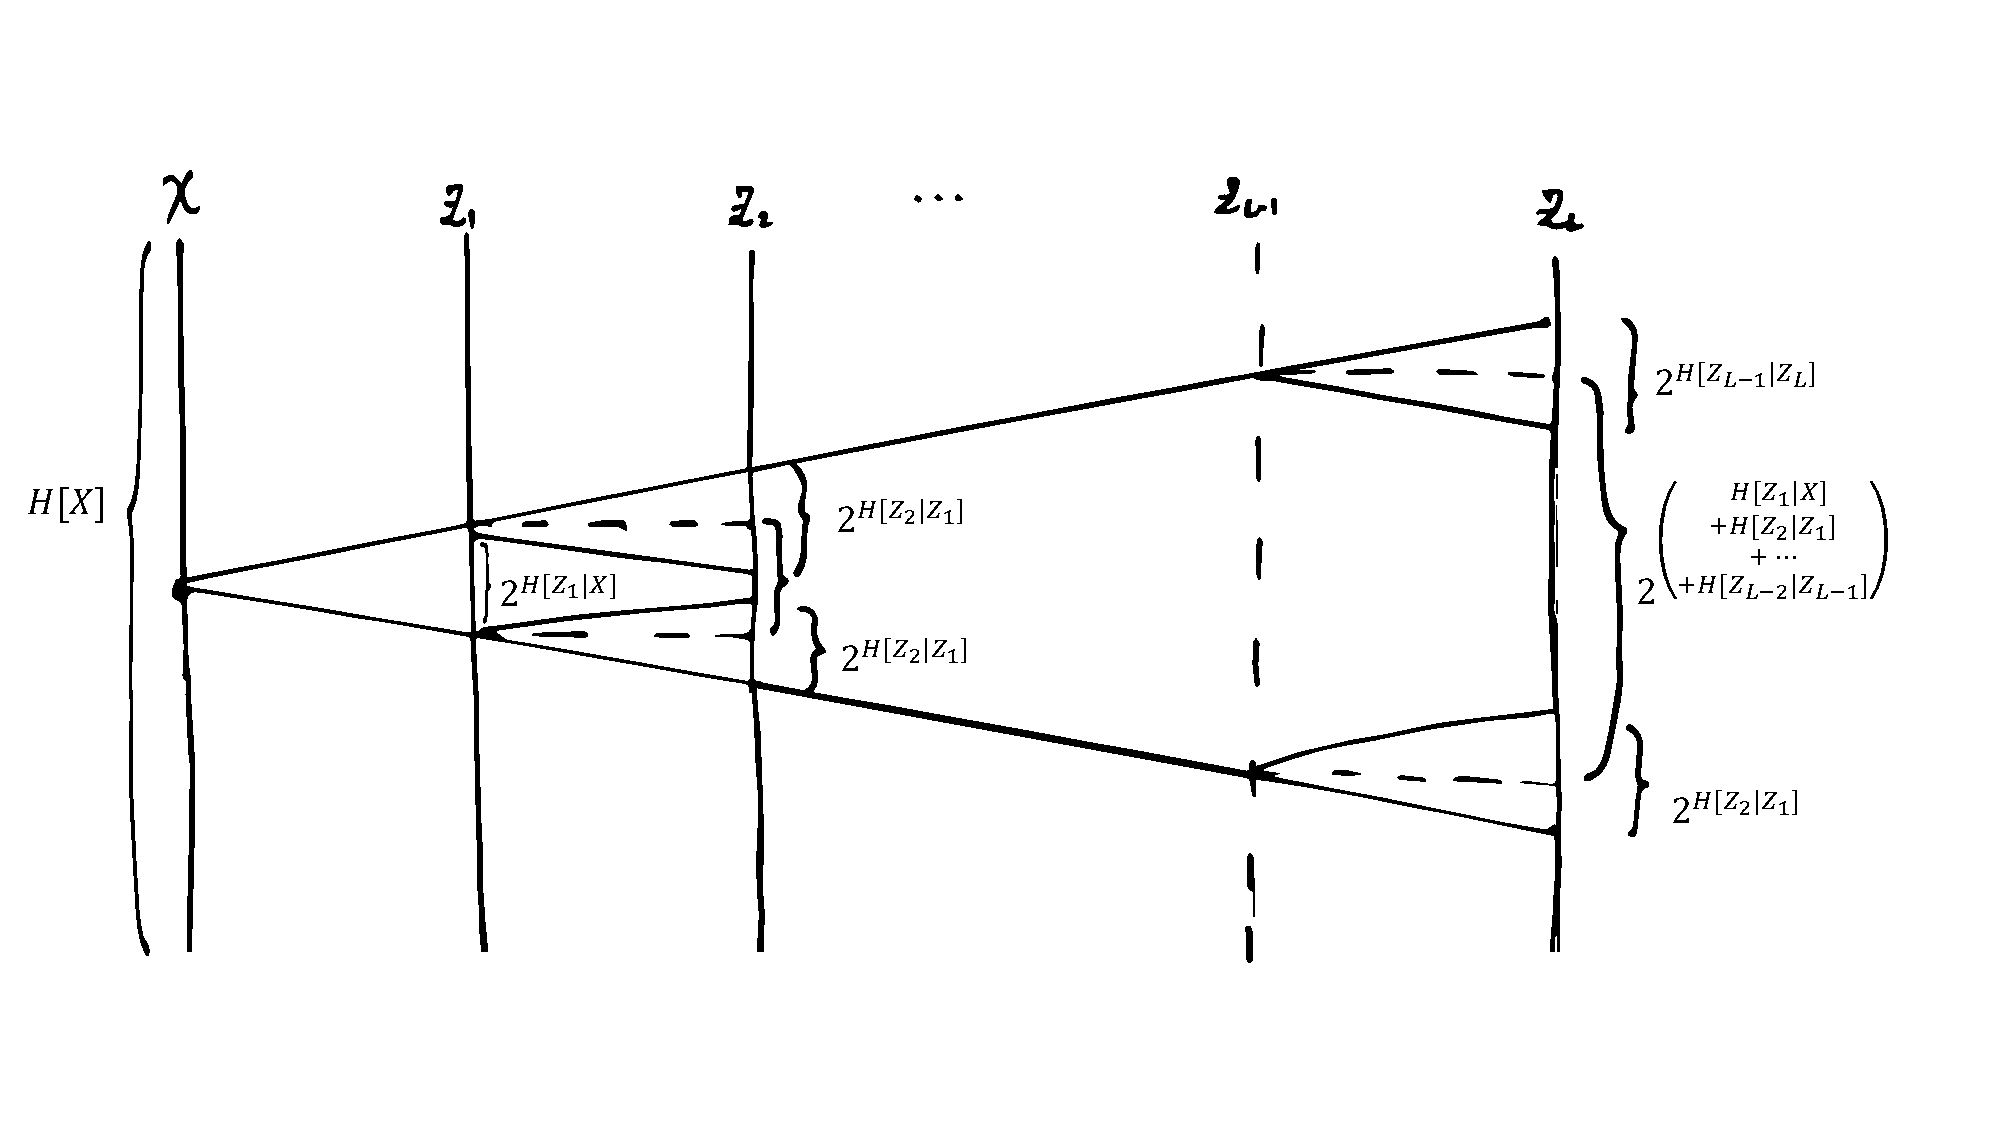
\includegraphics[width=\textwidth]{multi_layers}
	\caption{A visual explanation of corollary \ref{cor:stacking_layers}, stacking layers decrease the mutual information.}\label{fig:stacking_layers}
\end{figure}

Now, let us compare with the case of $L$ layers. Each layer acts as an encoder $q_i:\rvZ_{i-1} \to \rvZ_i$. The typical hypothesis space of $q_i$ depends on the cardinality of the possible values of $z_i$, which will depend on the size of the typical hypothesis space of $q_{i-1}$ (a one-to-one map): $|q_i^\epsilon| = \frac{|q_{i-1}^\epsilon|}{2^{H[\rvZ_i|\rvZ_{i-1}]}}$.

\begin{align}
	Q_{L} &= Q(\rvZ_{L} |\rvZ_{L-1}) \circ Q(\rvZ_{L -1}|\rvZ_{L-2}) \circ \cdots \circ Q(\rvZ_1|\rvX)\\
	\therefore \\
	|\sA_{Q_L}^\epsilon |&= \frac{2^{H[\rvX]}}{2^{(H[\rvZ_1|\rvX]+H[\rvZ_2|\rvZ_1]+\cdots + H[\rvZ_{L-1}|\rvZ_L])}}\\
	&= 2^{I[\rvZ_1|\rvX]-(H[\rvZ_2|\rvZ_1]+\cdots + H[\rvZ_{L-1}|\rvZ_L])}
\end{align}
We still need to show that $H[\rvZ_i|Z_{i-1}] \neq 0, i\in{1 \ldots \ell}, \rvX = Z_0$, \ie $I[X;Z_{L=1}]$ in $Q_1$ is bigger than $I[X;Z_L]$ in $Q_L$ even if $dim(\rvZ_L)$ is the same in both cases. Besides the dimension reduction, even if we disconsider the fact that with more nodes we can explicitly add more noise via dropout or other techinique, there are still the implicity increase of quantization noise caused by the added nodes. Therefore, $H[\rvZ_i|Z_{i-1}] >0$.
\begin{align}
	H[\rvZ_i|Z_{i-1}] >0 \to \left(|\sA_{Q_L}| < |\sA_{Q_1}| \right).
\end{align}

This is a direct consequence of corollary \ref{cor:stacking_layers}, $\left( I[\rvZ_L|\rvX]<I[\rvZ_1|\rvX] \right) \to \left(|\sA_{Q_L}| < |\sA_{Q_1}| \right)$.


For every bit in $(H[\rvZ_2|\rvZ_1]+\cdots + H[\rvZ_{L-1}|\rvZ_L])$, the hypothesis space is divided by 2. Thus, not only $|\sA_{Q_L}| < |\sA_{Q_1}|$, but $|\sA_{Q_L}| \ll |\sA_{Q_1}|$ (exponentially smaller).

\subsection{Sample bounds on empirical mutual information}



\subsection{The IB solution curve}
\begin{itemize}
	\item borja?
	\item non deterministic scenario
	\item deterministic scenario
	\item $\epsilon$-deterministic scenario
\end{itemize}
